The overall structure of the software system is designed to seamlessly support the palletizing tasks of the UR20 robot arm system. This layered design enables modular functionality, enhancing system adapability and ensuring each layer performs a unique function while simultaneously providing crucial information to the main PLC layer which manages data distribution. As the central interface, the PLC efficiently processes the flow of sata from each subsystem layer, allowing for smooth system integration and effective coordination across all layers. This architecture promotes reliable, dynamic operation, optimizing the UR20's performance in real-time palletizing tasks.
\begin{figure}[h!]
	\centering
 	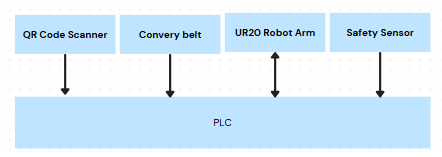
\includegraphics[width=0.60\textwidth]{images/layers}
 \caption{UR20 Architectural design diagram}
\end{figure}

\subsection{Layer 1: PLC Description}
The PLC will process most of the data through its peripherals, as seen in Figure 1. It is the primary interface between the different layers of the project. The built-in PLC will be configured with URScript, a Python-based scripting language in which vital functions will reside, such as the input function, the box offset algorithm, and finally, a position algorithm. The data flow will start with the input given by the Photo Eye scanner or the safety sensor, and the input functions will follow these two data paths. First being, an input given by the photo eye scanner will pass through the input function, which will then call the box offset algorithm to determine where the box is in 3D space given the location, which will go to the position algorithm and determine the motion necessary for the UR20 to satisfy this request. The safety algorithm will give the second path, which will trigger the input function and call the position algorithm to safely slow down the speed at which the UR20 is palletizing to create a safe work area for a cooperative application.

\subsection{Layer 2: Safety Sensor}
The Safety Sensor will determine if a human is in the area of the UR20 arm. If so, it will reduce the speed of the UR20 in order to create a safe work environment. This will be achieved with the use of a camera that will process the data in real-time with the use of computer vision, which will send a signal to the PLC which in turn will send a signal to the UR20 movement subsystem in order to maintain a safe speed for collaborative work.

\subsection{Layer 3: UR20 Robot Arm}
UR20 Arm consists of a vacuum gripper, the gripper controller, and the movement of the arm. The arm is the physical output of the software that resides in the PLC layer. Additionally, it contains a gripper grab/release controller (the controller for the air compressor), which will be turned on or off when needed to hold or drop a box. The commands given by the PLC will determine the position and orientation needed for the UR20 to place the box correctly.

\subsection{Layer 5: Conveyor Belt}
The conveyor belt system moves over pulleys driven by a motor. As the motor rotates, it propels the belt forward, allowing items placed on the belt to be conveyed along its length. The belt's speed can be adjusted to control the pace of movement. However, for this implementation, it will have two states: on or off. At the end of the conveyor belt, there will be a guide to reorient the boxes and a bracket in which the Photo Eye scanner will be placed.